\documentclass[../main.tex]{subfiles}

\usepackage{makecell}
\usepackage{amsmath}

\titleformat{\section}
  {\normalsize\bfseries}{\thesection}{1em}{\normalfont}

\pagestyle{empty}

\setcounter{chapter}{1}
\pagenumbering{arabic}
\setcounter{page}{7}

\newenvironment{blockquote}{%
  \par%
  \medskip
  \leftskip=3.5em\rightskip=2em%
  \noindent\ignorespaces}{%
  \par\medskip}


\begin{document}

\chapter{}
\label{cha:cha_2}


\section{}

\begin{lstlisting}[numbers=none]
>> q0 = 10;R = 50;L = 5;C = 1e-4;
>> t = linspace(0,.5);
>> q = q0*exp(-R*t/(2*L)).*cos(sqrt(1/(L*C)-(R/(2*L))^2)*t);
>> plot(t,q) 
\end{lstlisting}

\begin{figure}[H]
		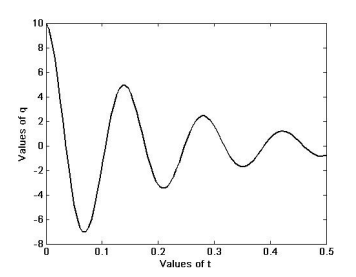
\includegraphics[width=0.5\linewidth]{fig_2_1}
		\label{fig:fig_2_1}
	\end{figure}

\section{}
\begin{lstlisting}[numbers=none]
>> z = linspace(-3,3);
>> f = 1/sqrt(2*pi)*exp(-z.^2/2);
>> plot(z,f)
>> xlabel('z')
>> ylabel('frequency')
\end{lstlisting}

\begin{figure}[H]
		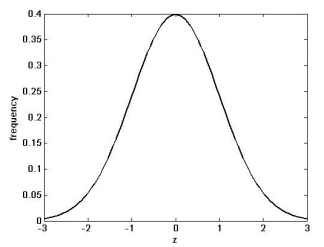
\includegraphics[width=0.5\linewidth]{fig_2_2}
		\label{fig:fig_2_ 2}
	\end{figure}
\section{}
\begin{enumerate}[label=\bfseries(\alph*)]
\item 
\begin{lstlisting}[numbers=none]
>> t = linspace(5,30,6) 

t =
 5 10 15 20 25 30 
\end{lstlisting}

\item

\begin{lstlisting}[numbers=none]
>> x = linspace(-3,3,7)

x =
 -3 -2 -1 0 1 2 3 
\end{lstlisting}
\end{enumerate}
\section{}
\begin{enumerate}[label=\bfseries(\alph*)]
\item
\begin{lstlisting}[numbers=none]
>> v = -2:.75:1

v =
 -2.0000 -1.2500 -0.5000 0.2500 1.0000 
\end{lstlisting}

\item
\begin{lstlisting}[numbers=none]
>> r = 6:-1:0

r =
 6 5 4 3 2 1 0 
\end{lstlisting}
\end{enumerate}
\section{}
\begin{lstlisting}[numbers=none]
>> F = [10 12 15 9 12 16];
>> x = [0.013 0.020 0.009 0.010 0.012 0.010];
>> k = F./x

k =
 1.0e+003 *
 0.7692 0.6000 1.6667 0.9000 1.0000 1.6000

>> U = .5*k.*x.^2

U =
 0.0650 0.1200 0.0675 0.0450 0.0720 0.0800

>> max(U)

ans =
 0.1200 
\end{lstlisting}
\bigbreak
\section{}
\begin{lstlisting}[numbers=none]
>> TF = 32:3.6:93.2;
>> TC = 5/9*(TF-32);
>> rho = 5.5289e-8*TC.^3-8.5016e-6*TC.^2+6.5622e-5*TC+0.99987;
>> plot(TC,rho) 
\end{lstlisting}
\begin{figure}[H]
		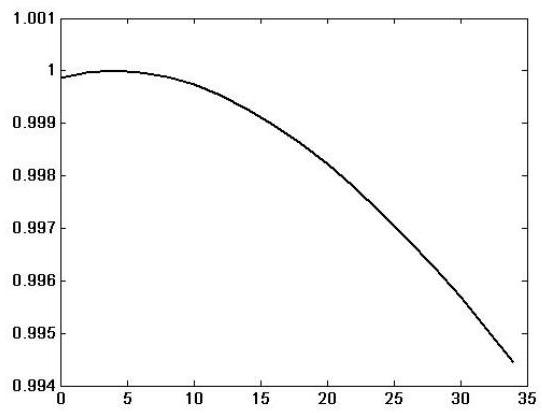
\includegraphics[width=0.5\linewidth]{fig_2_3}
		\label{fig:fig_2_ 3}
	\end{figure}
\section{}
\begin{lstlisting}[numbers=none]
>> A = [.035 .0001 10 2;
.02 .0002 8 1;
.015 .001 20 1.5;
.03 .0007 24 3;
.022 .0003 15 2.5]

A =
 0.0350 0.0001 10.0000 2.0000
 0.0200 0.0002 8.0000 1.0000
 0.0150 0.0010 20.0000 1.5000
 0.0300 0.0007 24.0000 3.0000
 0.0220 0.0003 15.0000 2.5000

>> U = sqrt(A(:,2))./A(:,1).*(A(:,3).*A(:,4)./(A(:,3)+2*A(:,4))).^(2/3)

U =
 0.3624
 0.6094
 2.5167
 1.5809
 1.1971
\end{lstlisting}
\bigbreak
\section{}
\begin{lstlisting}[numbers=none]
>> t = 10:10:60;
>> c = [3.4 2.6 1.6 1.3 1.0 0.5];
>> tf = 0:70;
>> cf = 4.84*exp(-0.034*tf);
>> plot(t,c,'s',tf,cf,'--') 
\end{lstlisting}
\begin{figure}[H]
		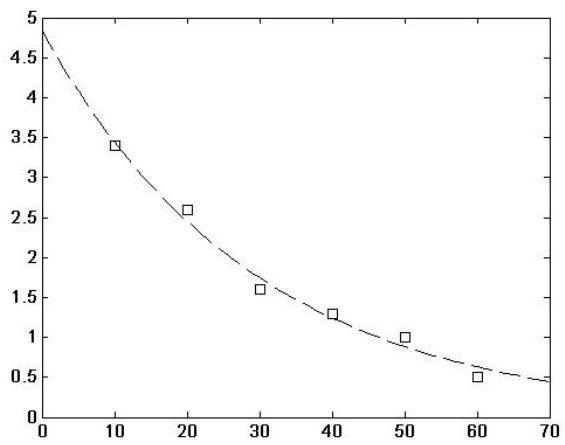
\includegraphics[width=0.5\linewidth]{fig_2_4}
		\label{fig:fig_2_ 4}
	\end{figure}
\section{}
\begin{lstlisting}[numbers=none]
>> t = 10:10:60;
>> c = [3.4 2.6 1.6 1.3 1.0 0.5];
>> tf = 0:70;
>> cf = 4.84*exp(-0.034*tf);
>> semilogy(t,c,'s',tf,cf,'--') 
\end{lstlisting}
\begin{figure}[H]
		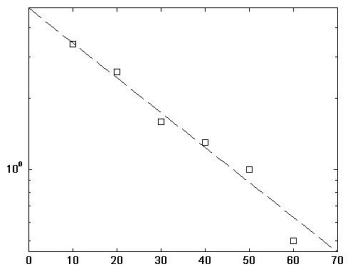
\includegraphics[width=0.5\linewidth]{fig_2_5}
		\label{fig:fig_2_ 5}
	\end{figure}
\section{}
\begin{lstlisting}[numbers=none]
>> v = 10:10:80;
>> F = [25 70 380 550 610 1220 830 1450];
>> vf = 0:100;
>> Ff = 0.2741*vf.^1.9842;
>> plot(v,F,'d',vf,Ff,':') 
\end{lstlisting}
\begin{figure}[H]
		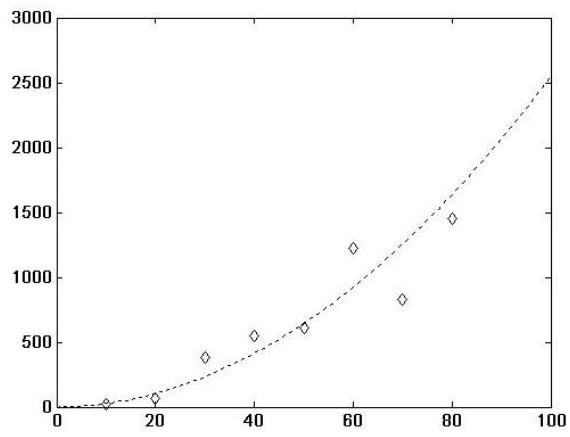
\includegraphics[width=0.5\linewidth]{fig_2_6}
		\label{fig:fig_2_ 6}
	\end{figure}
\section{}
\begin{lstlisting}[numbers=none]
>> v = 10:10:80;
>> F = [25 70 380 550 610 1220 830 1450];
>> vf = 0:100;
>> Ff = 0.2741*vf.^1.9842;
>> loglog(v,F,'d',vf,Ff,':') 
\end{lstlisting}
\begin{figure}[H]
		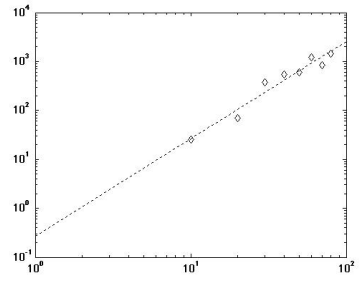
\includegraphics[width=0.5\linewidth]{fig_2_7}
		\label{fig:fig_2_ 7}
	\end{figure}


\section{}
\begin{lstlisting}[numbers=none]
>> x = linspace(0,3*pi/2);
>> c = cos(x);
>> cf = 1-x.^2/2+x.^4/factorial(4)-x.^6/factorial(6);
>> plot(x,c,x,cf,'--')
\end{lstlisting}
\begin{figure}[H]
		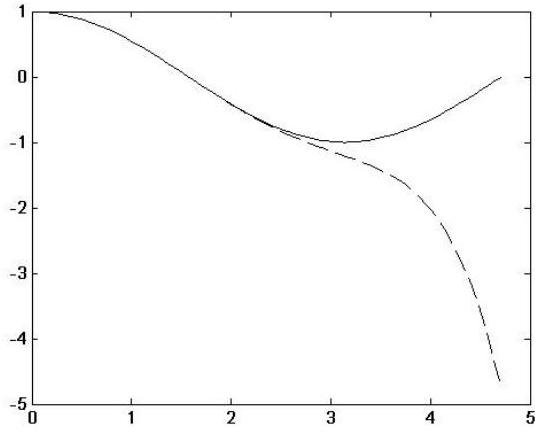
\includegraphics[width=0.5\linewidth]{fig_2_8}
		\label{fig:fig_2_ 8}
	\end{figure}
\end{document}

